\documentclass[12pt]{article}
\usepackage{geometry}                % See geometry.pdf to learn the layout options. There are lots.
\geometry{letterpaper}                   % ... or a4paper or a5paper or ... 
%\geometry{landscape}                % Activate for for rotated page geometry
\usepackage[parfill]{parskip}    % Activate to begin paragraphs with an empty line rather than an indent
\usepackage{graphicx}
\usepackage{amssymb}
\usepackage{epstopdf}
\DeclareGraphicsRule{.tif}{png}{.png}{`convert #1 `dirname #1`/`basename #1 .tif`.png}

%usepackage{color}
\usepackage[usenames,dvipsnames]{color}
\usepackage{fancyvrb}
\usepackage{listings}
\usepackage{caption}
\usepackage{url}

% include the lines below to use a nicer fixed-width font than the default one
% \usepackage{fontspec}

%\setmonofont[Scale=0.8]{Consolas}

\lstset{
		fancyvrb=true,
		basicstyle=\small\tt,
		keywordstyle=\color{blue},
		identifierstyle=,
		commentstyle=\color{Gray},
		stringstyle=\color{red},
		showstringspaces=false,
		tabsize=3,
		numbers=left,
		captionpos=b,
		numberstyle=\tiny,
		breaklines=true
%stepnumber=4
}


\title{Repast HPC Manual}
\author{Nick Collier}
\begin{document}
\maketitle
\section{Introduction}

Repast for High Performance Computing (Repast HPC) is an agent-based modeling and simulation
(ABMS) toolkit for high performance distributed computing platforms. Repast HPC is based on the principles and
concepts development in the Repast Simphony toolkit. Repast HPC is written in C++ using MPI for
parallel operations. It also makes extensive use of the boost (http://boost.org) library.

Repast HPC is intended for users with:
\begin{itemize}
\item
Basic C++ expertise
\item 
Access to high performance computers 
\item
A simulation amenable to a parallel computation. Simulations that consist of many local interactions are typically good candidates.
\end{itemize}�
Models can be written in C++ or with  a ``Logo-style" C++.

\section{Core Concepts}
\subsection{Repast Simphony}
Repast HPC implements the core Repast Simphony concepts and features.

Agents are implemented as 
Objects, in the case of Repast HPC, as C++ classes. An agents' state is represented by the field variables of those classes and
agent behavior by methods in those classes. For example, a bird agent in a flock simulation might be implemented as a C++ Bird class with field variables for its heading and speed. A fly method might move the bird some distance according the speed and heading.
\begin{minipage}[h]{\textwidth}
\lstset{language=c++,caption=An Example Agent}
\begin{lstlisting}
class Bird {

private:
	float heading;
	float speed;

public:
	...
	void fly();
}
\end{lstlisting}
\end{minipage}

The simulation proceeds using a schedule. Each iteration of the simulation, the next event is popped of the schedule queue and 
executed. Repast HPC implements a dynamic discrete-event scheduler with conservative synchronization. The user schedules
events to occur at a specific {\em tick}  and the ticks determine the relative order in which the events occur. For example, if event A
is scheduled to occur at tick 3, and event B is scheduled for tick 5, then A will execute before B.

A {\em Context} is used to encapsulate the population of agents. The Context implements set semantics so it only contains a single instance of each agent. As agents are created they are added to a Context and when they die, they are removed from a Context. The Context has {\em Projections} associated with it. A Projection imposes a relational structure on the agents in the Context. For example, a grid projection puts agents into a grid matrix type structure where each agent occupies some cell location in the grid. A network projection allows agents to have network link relationships with each other. An agent in a context automatically participates in the projections associated with that Context. When an agent is added to the Context, it becomes a member of the projections associated with the context. For example, if a Context has a network projection then any agents added to the Context become vertices in the network projection. Repast HPC implements 3 types of projections: A grid, a continuous space and a network.

A Repast HPC simulation is thus composed of agents, one or more contexts containing these agents, and zero or more projections. The user is responsible for writing the agent code. Repast HPC provides the context and projection implementations.  Simulation execution typically consists of getting the next scheduled event that the user has scheduled, and executing that event. The event will invoke agent behavior that uses one or more of the projections. For example, every iteration of a simulation, each agent might make network links, or poll the agents in neighboring grid cells.

\subsection{Parallel Simulation}
\subsubsection{Parallel Agents}
RepastHPC is designed for a parallel environment in which many processes are running in parallel and memory is {\em not} shared  across processes. The agents themselves are distributed across processes. Each process is responsible for the agents {\em local} to that process. An agent is local to process when the process executes the code that represents the local agent's behavior. Copies of {\em non-local} agents may reside on a process, allowing agents to be shared across processes. Local agents can then interact with these copies. 

For example, a user creates a simulation distributed across 2 process, P1 and P2. Each process creates 10 agents and has its own schedule which executes events. These events ultimately resolve to method calls on the 10 agents on that process. The 10 agents on P1 are local to P1. Only code executing on P1 changes their agent state. Similarly, the 10 agents on P2 are local to P2. Only code executing on P2 changes their agent state. P1 then requests a copy of agent A2 from P2. The Context on P1 now contains the copy of A2. A2 is non-local with respect to P1. The code that runs on P1 should not change the state of A2. Agents on P1 can query the state of A2 when executing their behavior, but the copy of A2 remains unchanged. Of course, the original A2 may change on P2 and in that case, Repast HPC can synchronize the state change between processes.

In order for agents to be distinguished from each other, both in a context and across processes, each agent must have a unique id. This id is represented in the AgentId class.

\lstset{language=c++,caption=AgentId Class,label=lst:nicecode}
\begin{lstlisting}
class AgentId {
   ....

public:
	/**
	 * Creates an AgentId. The combination of the first
	 * three parameters should uniquely identify the agent.
	 *
	 * @param id the agent's id
	 * @param startProc the rank of the agent's starting process
	 * @param agentType the agent's type (user defined)
	 * @param currentProc the rank where the agent is a local agent
	 */
	AgentId(int id, int startProc, int agentType, int currentProc = -1);

	virtual ~AgentId();

	/**
	 * Gets the id component of this AgentId.
	 *
	 * @return the id component of this AgentId.
	 */
	int id() const;

	/**
	 * Gets the starting rank component of this AgentId.
	 *
	 * @return the starting rank component of this AgentId.
	 */
	int startingRank() const;
	
	/**
	 * Gets the agent type component of this AgentId.
	 *
	 * @return the agent type component of this AgentId.
	 */
	int agentType() const;
	/**
	 * Gets the current process rank of this AgentId. The current rank
	 * identifies which process the agent with this AgentId is
	 * currently on.
	 *
	 * @return the current process rank of this AgentId.
	 */
	int currentRank() const;
	/**
	 * Sets the current process rank of this AgentId. The current rank
	 * identifies which process the agent with this AgentId is
	 * currently on.
	 *
	 * @param val the current process rank
	 */
	void currentRank(int val);
	/**
	 * Gets the hashcode for this AgentId.
	 *
	 * @return the hashcode for this AgentId.
	 */
	std::size_t hashcode() const;
}

\end{lstlisting}
An AgentId has 4 components: 

\begin{itemize}
\item
id - an user specified numeric id. All agents created on the same process should have a different id.
\item
agent type - an int signifying the type of the agent. An agent's type corresponds to the agent's C++ class. For example,
Bird may have type 0 and Wolf type 1.
\item
starting rank - the rank of the process on which the agent was created.
\item
current rank - the rank of the process that the agent is local to. When an agent is created is starting rank and current rank will be identical. However, if the agent moves, {\em not copied}, between processes then the current rank will updated to match the
new process.
\end{itemize}�
The AgentId also returns a hashcode() that can be used in unordered stl maps. The structs HashId and AgentHashId found in AgentId.h can be used to parameterize such maps or sets for use with agents and AgentIds.

All RepastHPC agents are required to implement the Agent interface which simple provides the AgentId for that agent.

\lstset{language=c++,caption=Agent Interface,label=lst:nicecode}
\begin{lstlisting}
class Agent {
public:
	virtual ~Agent() {}
	virtual AgentId& getId() = 0;
	virtual const AgentId& getId() const = 0;
};
\end{lstlisting}

\subsubsection{Cross-process Communication and Synchronization}
Because Repast HPC simulations are distributed across multiple processes, cross-process communication and synchronization of the simulation state across those processes is often necessary. In particular cross-process communication and synchronization are necessary:

\begin{itemize}
\item
when one process requires copies of agents from another process. This is often necessary in order to ``stitch" the global pan-process model into a coherent whole.
\item
 when a process contains non-local agents (or edges) that have been copied from another process, and the copies must be updated with the latest state from the original.
 \item
 when grid and space buffers need to be updated. See below for the details of grid and space buffers.
 \item
 when an agent must be moved completely from one process to another. This can occur as the result of grid movement as explained later below.
 \end{itemize}
 Repast HPC automates much of this, but the programmer must provide serialization type code extract the agent state and package it for transfer and then unpack the transferred package and create or update the appropriate agent from it. This packing and unpacking is known in RepastHPC  as the {\em Package} pattern. It occurs for all sorts of synchronization although the details may differ depending on the type of synchronization (e.g. copying agents the first time vs. updating existing copied agents). 
  
 The Package pattern consists of a Package that contains the state to communicate to another processes, a Provider that provides a Package given an agent or edge, and a Receiver that receives the Package, unpacks it and creates or updates an agent or edge from the Package. An example of the Package pattern follows. In this case, an agent is being copied from one process to another, and so the Receiver creates a new agent rather than updating an existing one.

\lstset{language=c++,caption=The Agent,label=lst:nicecode}
\begin{lstlisting}
class Human {
private: bool _infected;
AgentId id;
public: Human(AgentId id, bool infected) :
	 _infected(infected), _id(id){} 
};
\end{lstlisting}
The agent here is a Human from the example Zombies model. A  human's state is composed of its id and whether or not it is infected. Taken together these two fully describe a Human. The package then needs to encapsulate this state. 

\lstset{language=c++,caption=The Package,label=lst:nicecode}
\begin{lstlisting}
struct HumanPackage {
template<class Archive> 
void serialize(Archive& ar, const unsigned int version) {
	ar & id;
	ar & rank;
	ar & type; 
	ar & infected;
}
	
int id, rank, type; bool infected;
repast::AgentId getId() const { 
	return repast::AgentId(id, proc, type);
};
\end{lstlisting}
The HumanPackage contains the unique components of a Human's AgentId and the bool infected. All packages are required to implement

\captionsetup{labelformat=empty,labelsep=none}
\lstset{language=c++,caption=, numbers=none}
\begin{lstlisting}
repast::AgentId getId() const;
\end{lstlisting}
in order to identify the agent the package is for. And so the Human package does so here. Lastly the HumanPackage implements
 
\lstset{language=c++, numbers=none}
\begin{lstlisting}
template<class Archive> 
void serialize(Archive& ar, const unsigned int version)
\end{lstlisting}

This method performs that actual serialization an Archive. It is this Archive that is then passed via MPI to the other process. Repast HPC uses boost MPI for almost all of its MPI related function. More on it can be found at \url{http://www.boost.org/doc/libs/1_44_0/doc/html/mpi.html} and more on boost serialization at \url{http://www.boost.org/doc/libs/1_44_0/libs/serialization/doc/index.html}. The general idea is quite simple though. Any types that are serializable by boost can be serializes using "ar \& " followed by the variable. Types can be made serializable using the serialize method above.

\begin{minipage}[h]{\textwidth}
\captionsetup{labelformat=simple,labelsep=colon}
\lstset{language=c++,caption=The Provider, numbers=left}
\begin{lstlisting}
void Provider::providePackage(Human* agent,
	 std::vector<HumanPackage>& out) {
	 
	AgentId id = agent->getId(); 
	HumanPackage package = {id.id(), id.startingRank(),
		id.agentType(),agent->infected()}; 
	out.push_back(package);
}
\end{lstlisting}
\end{minipage}
The Provider  takes a Human and creates a package from its state. Providers will typically add the created package to a vector as is done here. 

\begin{minipage}[h]{\textwidth}
\captionsetup{labelformat=simple,labelsep=colon}
\lstset{language=c++,caption=The Receiver,label=lst:receiver, numbers=left}
\begin{lstlisting}
Human* Receiver::createAgent(HumanPackage& package) {
 	return new Human(package.getId(), package.infected));
}
\end{lstlisting}
\end{minipage}
The Receiver takes  the package and makes a Human agent out of it. 


This Package pattern applies both to simulations written in straight C++ and those written in the logo-like C++. The details and signatures of the provider and receiver will vary slightly but the idea remains the same.


\section{Repast HPC Simulation Components}
This section describes the simulation components implements by Repast HPC, focusing in particular on how they work in the parallel distributed environment. Additional details about the components can be found in the API documentation. These components are used when writing a simulation using C++, and to a much lesser extent when writing logo-like C++ simulations, especially for the parallel projections.

\subsection{Repast Process}
The Repast Process component together with its associated functions manages inter-process communcation and non-local (copied) agent synchronization. The RepastProcess is implemented as a singleton (one per process). It can be retrieved with

\captionsetup{labelformat=empty,labelsep=none}
\lstset{language=c++,caption=, numbers=none}
\begin{lstlisting}
RepastProcess* rp = RepastProcess::instance();
\end{lstlisting}

It has methods for getting the total number of processes in the simulation and getting the current process. Associated functions allow the user to request agents from other processes. These agents then become non-local copied agents in the calling process. 

\captionsetup{labelformat=empty,labelsep=none}
\lstset{language=c++,caption=, numbers=none}
\begin{lstlisting}
  template<typename T, typename Content, typename Provider, typename Updater, typename AgentCreator>
  void requestAgents(SharedContext<T>& context, AgentRequest& request, Provider& provider, Updater& updater, AgentCreator& creator
      , std::string setName = DEFAULT_AGENT_REQUEST_SET, AGENT_IMPORTER_EXPORTER_TYPE setType = DEFAULT_ENUM_SYMBOL
#endif
);
\end{lstlisting}

This uses the Package pattern to package, provide and receive the agents. The AgentRequest encapsulates the request and the context is the simulation context (as described above).  (The capitalized terms relate to an optimization strategy in which the agents are requested as a set, and the set is assigned a name by which this group of agents can later be referenced.) An example,

\captionsetup{labelformat=simple,labelsep=colon}
\lstset{language=c++,caption=Example Agent Request,label=lst:provider, numbers=left}
\begin{lstlisting}
AgentRequest request(RepastProcess::instance()->rank()); 
// get 10 random agents from other process 
for (int i = 0; i < 10; i++) {
  	AgentId id = createRandomOtherRankId(); 
  	request.addRequest(id);
} 
repast::RepastProcess::instance()->requestAgents<AgentType, AgentPackageContent, ProviderType, UpdaterType, CreatorType>(context, request, *this, *this, *this);
\end{lstlisting}
An AgentRequest is created, passing the process rank of the process making the request in the constructor. The requested ids are then added to the request. Then the request is made. Repast HPC will call the providers on the appropriate processes to provide the Packages that encapsulate the requested agents, and transfer these Packages to the receivers. The receivers will create Agents from these and Repast HPC will add those to the context. Note that in this example the Provider, Updater, and Creator are all the same class (the class making the request).

Agent state synchronization works similarly except that rather than creating new agents, the receiver is expected to update existing agents from the Package contents.
\captionsetup{labelformat=empty,labelsep=none}
\lstset{language=c++,caption=, numbers=none}
\begin{lstlisting}
  template<typename Content, typename Provider, typename Updater>
  void synchronizeAgentStates(Provider& provider, Updater& updater
   , std::string setName = REQUEST_AGENTS_ALL
);
\end{lstlisting}

(The setName parameter refers to the possibility of updating the agent states only of a named set of agents, as a potential optimization.)

The RepastProcess component also synchronizes the status of an agent. If an agent has been removed from the simulation (e.g. ``died") then any processes with a copy of it must be informed of its new status. Similarly, if an agent migrates to another process and becomes local to a new process then its status must be synchronized.
\captionsetup{labelformat=empty,labelsep=none}
\lstset{language=c++,caption=, numbers=none}
\begin{lstlisting}
template<typename T, typename Content, typename Provider, typename AgentCreator>
void RepastProcess::syncAgentStatus(SharedContext<T>& context, Provider& provider, AgentCreator& creator) 
\end{lstlisting}

Additional details about these methods and functions as well as the template type requirements can be found in the API documentation.




\subsection{Parallel Scheduling}
A described above, Repast HPC uses a discrete event scheduler to iterate the simulation forward. Each process has its own discrete-event schedule. TThe schedules are tightly and conservatively synchronized across processes (i.e., all processes execute the same tick). Each iteration of the schedule loop, each schedule determines the next tick (time step) that should be executed. Each schedule only executes events scheduled for a global minimum next tick which is determined using MPI's 'all reduce� on the set of local next ticks. This is largely invisible to the user though. The user just schedules events where are typically agent behaviors and data collection. Repast HPC handles any necessary synchronization.

\subsubsection{Scheduling an Event}
The RepastProcess provides access to the ScheduleRunner. The ScheduleRunner API allows the programmer to schedule events to execute at:
\begin{itemize}
\item
At a specific time (tick) 
\begin{lstlisting}
ScheduledEvent* scheduleEvent(double at,
	 Schedule::FunctorPtr func);
\end{lstlisting}
\item
Starting a specific time (tick) and repeating at some specified interval
\begin{lstlisting}
ScheduledEvent* scheduleEvent(double start, double interval, Schedule::FunctorPtr func);
\end{lstlisting}
\item
At the end of a simulation run
\begin{lstlisting}
void scheduleEndEvent(Schedule::FunctorPtr func);
\end{lstlisting}
\end{itemize}
Additional methods schedule the tick at which to stop the simulation and to preemptively stop the simulation. See the ScheduleRunner API docs for details.

The actual item scheduled for execution is a method call on some particular object instance. This method call is wrapped by some necessary objects. For example,
\captionsetup{labelformat=simple,labelsep=colon}
\lstset{language=c++,caption=Scheduling Example,label=lst:provider, numbers=left}
\begin{lstlisting}
ScheduleRunner& runner = RepastProcess::instance()->
	getScheduleRunner();
runner.scheduleEvent(1, 1, 
	Schedule::FunctorPtr(new MethodFunctor<MyModel> (myModel, 
	&MyModel::go)));
\end{lstlisting}
This schedules the execution of the {\em go} method on an instance of a MyModel class. The go method will be executed at tick 1 and every tick thereafter (an interval of 1). (Note that typical simulations have one class that it responsible for setup and initialization of the schedule. The MyModel here is just such a class.)All scheduled methods need to be wrapped in a MethodFunctor templated with the type that contains the method. The MethodFunctor is then wrapped by a Schedule::FunctorPtr. 

\subsection{SharedContext}
The SharedContext is a Context implementation specialized for the parallel distributed environment. Each process must contain at least on instance of a SharedContext. The SharedContext contains all the local and non-local agents currently on that process. A SharedContext is templated with the type of the agent(s) it contains. If it contains multiple types, the then template type is a shared base class and the agent type component of the AgentId can be used to determine the concrete class type. As a collection of agents, a SharedContext has a variety of methods for adding and retrieving them. For example,

\captionsetup{labelformat=empty,labelsep=none}
\lstset{language=c++,caption=, numbers=none}
\begin{lstlisting}
bool addAgent(T* agent);
T* getAgent(const AgentId& id);
void getRandomAgents(const int count, std::vector<T*>& agents);
void removeAgent(const AgentId id);
void removeAgent(T* agent);
\end{lstlisting}

There also iterators for iterating over both the local and all agents as well as agents by type.
\captionsetup{labelformat=empty,labelsep=none}
\lstset{language=c++,caption=, numbers=none}
\begin{lstlisting}
const_local_iterator localBegin() const;
const_local_iterator localEnd() const;
const_iterator begin() const;	
const_iterator end() const;
const_bytype_iterator byTypeBegin(int typeId) const;
const_bytype_iterator byTypeEnd(int typeId) const;
\end{lstlisting}

Lastly, Projections can be associated with the SharedContext by adding them to the SharedContext. They can also be retrieved by name.
\captionsetup{labelformat=empty,labelsep=none}
\lstset{language=c++,caption=, numbers=none}
\begin{lstlisting}
void addProjection(Projection<T>* projection);
Projection<T>* getProjection(const std::string& name);
\end{lstlisting}
See the API docs for Context and SharedContext for more details.

\subsection{Parallel Projections}
Parallel projections impose relational structure on members of contexts. In addition to the API relevant to their the structure (e.g. Network::addEdge), parallel projections provide functionality for composing a pan-process projection from smaller local ones. Smaller local grids create a pan-process grid through the use of a buffer Smaller local networks create a pan-process network though cross-process links, and the creation of complementary links. Parallel projections are added by name to a SharedContext during their setup.  Projections can be retrieved by name from the SharedContext. Any agent added to the SharedContext is automatically added to its associated projections.

\subsubsection{Shared Networks}
The SharedNetwork provides typical network functionality such as creating and removing edges, finding node successors and predecessors, iterators over vertices and edges.
\captionsetup{labelformat=empty,labelsep=none}
\lstset{language=c++,caption=, numbers=none}
\begin{lstlisting}
E* addEdge(V* source, V* target);
E* addEdge(V* source, V* target, double weight);
E* findEdge(V* source, V* target);
void successors(V* vertex, std::vector<V*>& out);
void predecessors(V* vertex, std::vector<V*>& out);
void adjacent(V* vertex, std::vector<V*>& out);
\end{lstlisting}
where V and E are template parameters, identifying the vertex (i.e. agent) and edge types respectively. The default edge type is RepastEdge and any user edge types should extend the RepastEdge class.

The network represented by the SharedNetwork class is distributed across processes. Each process manages some smaller part of the larger pan-process network. The smaller parts are stitched together by the user using shared (i.e. agents) and shared edges. 

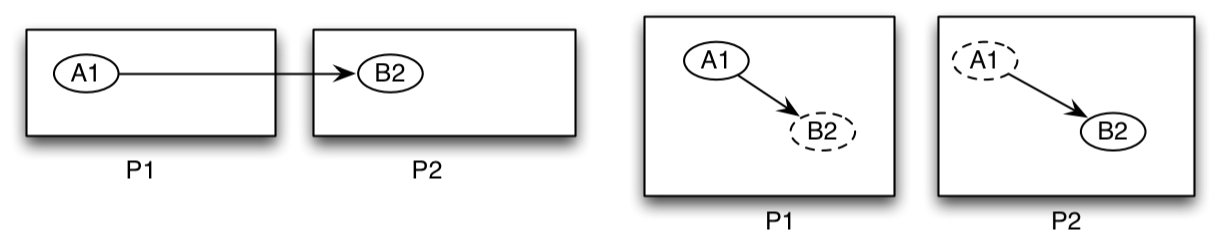
\includegraphics[width=150mm]{net.png}

\subsubsection{Shared Grids and SharedSpaces}
Shared Grid and Shared Space projections provide the typical ABMS grid and space functionality for discrete grids and continuous spaces. Namely, moving agents to some particular grid or space location, getting the agent or agents at a particular location, and getting the location of some particular agent.

\captionsetup{labelformat=empty,labelsep=none}
\lstset{language=c++,caption=, numbers=none}
\begin{lstlisting}
bool moveTo(const AgentId& id, const Point<GPType>& pt);
T* getObjectAt(const Point<GPType>& pt) const;
void getObjectsAt(const Point<GPType>& pt, 
	std::vector<T*>& out) const;
bool getLocation(const T* agent,
	 std::vector<GPType>& out) const;
\end{lstlisting}
\texttt{GPType} is the coordinate type for a grid or spaces location. For a discrete grid the \texttt{GPType}  will be an int. For a continuous space it will be a double.

The discrete grid and continuous space code derives from a common base class and they are largely separated through the use of particular template parameters. Four typical types have been defined as typedefs with default template arguments in the SharedGrids struct.
\begin{enumerate}
\item
SharedWrappedDiscreteSpace - a discrete periodic grid, that is, a grid wrapped to become a torus.
\item
SharedStrictDiscreteSpace - a discrete grid with strict, non-wrapped borders.
\item
SharedWrappedContinuousSpace - a continuous space wrapped into a torus.
\item
SharedStrictContinuousSpace - a continuous space with strict, non-wrapped borders.
\end{enumerate}

As with the SharedNetwork, shared grids and spaces are distributed across processes. Each process is responsible for a particular section of a larger pan-process grid. Each subsection has a user-defined buffer that specifies how much of the grid to share with other processes.

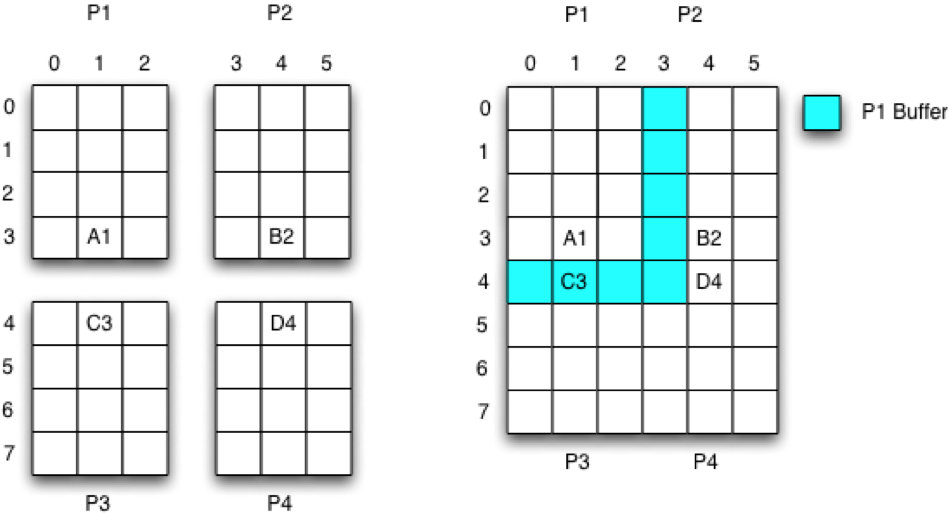
\includegraphics[width=150mm]{grid.png}

Here there are 4 processes, each responsible for a subsection of the grid. The entire grid runs from (0,0) x (5,7). Process P1 is responsible for the subsection (0,0) x (2, 3), P2 for (3,0) x (5,3) and so on. The buffer has a value of 1, so P1, for instance, contains a buffered area that includes all of column 3 from P2 and row 4 from P3. In this way, the larger pan-process grid is stitched together by overlapping the smaller subsections. Grid and space buffers are synchronized using the Package type pattern the \texttt{synchBuffer} method called on the grid or space that is being synchronized. See the API docs for more info.

Repast HPC is designed so that agents local to a process have a location that is within the bounds of the process' grid or space subsection. For example, all the agents local to P1 are expected to have a location within (0,0) x (2, 3). If an agent moves off the local grid, then that agent will be migrated to the process whose grid subsection the agent has moved into. This migration will occur when the agent's status is updated using the `synchronize agent status' method described above.

\subsection{Synchronizing Projections}

RepastProcess includes a method that, when called, synchronizes projection information. The method signature is:

\captionsetup{labelformat=empty,labelsep=none}
\lstset{language=c++,caption=, numbers=none}
\begin{lstlisting}
  template<typename T, typename Content, typename Provider, typename Updater, typename AgentCreator>
  void synchronizeProjectionInfo(SharedContext<T>& context, Provider& provider, Updater& updater, AgentCreator& creator,
      EXCHANGE_PATTERN exchangePattern = POLL
  #ifdef SHARE_AGENTS_BY_SET
      , bool declareNoAgentsKeptOnAnyProcess = false
  #endif
);
\end{lstlisting}

In Repast HPC 1.0.1, independent synchronization calls were provided for each projection. Repast HPC 2.0 replaces this with the new synchronizeProjectionInformation method. When called this method:

\begin{enumerate}
\item removes all non-local agents that are on the process that are not needed
\item updates all other processes with new projection information pertaining to agents that either do or should exist as non-local agents on other processes (and receives the same from the other processes)
\end{enumerate}

For example, consider a simulation that has a network projection and a spatial projection. A given process should have all of its local agents, plus all of the agents in the buffer zones of the surrounding processes, plus all of the agents to which it is connected in the network. Calling the synchronize method will result in these agents being present on the process. Non-local agents that are not needed are removed. For example, suppose an agent from another process was on the local process because it was connected to a local agent via a network connection; suppose, however, that this connection were eliminated on the other process. After synchronization, this agent would no longer be on the local process. Similarly, suppose a non-local agent were present because it was in an adjacent process's buffer zone, but since the last synchronization, the agent has moved out of the buffer zone. When synchronization is called this agent will no longer be present on the local process.

An important aspect of this new synchronization strategy is that all non-local agents arrive on a process with all of their projection information. In the preceding example, the agent that was present on the local process because of a network connection would still have had its spatial location available: it would be possible for the local agent that is the source of the network connection to have obtained the spatial location of the non-local agent to which it was connected, even though that agent's position might be many processes away in simulation space.

\subsection{Data Collection}
Repast HPC supports two types of data collection:
\begin{enumerate}
\item
Aggregate Data Collection. Aggregate data collection uses MPI's reduce functionality to aggregate (sum, min, max, etc)data across processes and write the result to single file. The user specifies named numeric data sources and the reduction operation to apply to each of them across all processes. The resulting output records the tick at which the data was collected and the result of the reduce operation on each named data source.  Output can be written in netCDF or plain text format. Data collection tick is written to a �tick� column. Each data source result is written to its own column.
\item
Non-Aggregate Data Collection. Non-Aggregate data collection is similar to aggregate data collection but no reduce operation is specified. Output is to single file and includes a column variable specifying the process rank that produced the data.
\end{enumerate}

Data is captured in a Dataset. The steps to creating one are:
\begin{enumerate}
\item
Create a DataSetBuilder
\item
Add Data Sources to the builder
\item
Create the DataSet from the builder
\item
Schedule the DataSet recording and writing.
\end{enumerate}�
There are different builders for the different data formats, netCDF and plain text. The process and methods are the same but the netCDF ones will be prefixed with NC while the plain text will be prefixed with SV (for Separated Value). The following is an example using the netCDF format.

\begin{minipage}[h]{\textwidth}
\captionsetup{labelformat=empty,labelsep=none}
\lstset{language=c++,caption=, numbers=left}
\begin{lstlisting}
// create a builder for netcdf aggregate data collection
NCDataSetBuilder builder("./output/data.ncf", RepastProcess::instance()->getScheduleRunner().schedule());
// this is the data source
InfectionSum* infectionSum = new InfectionSum(this);
builder.addDataSource(repast::createNCDataSource("number_infected", infectionSum, std::plus<int>()));

DataSet* dataSet = builder.createDataSet();
// schedule the record and write on the dataset
ScheduleRunner& runner = RepastProcess::instance()->getScheduleRunner();
runner.scheduleEvent(1.1, 1, Schedule::FunctorPtr(new MethodFunctor<repast::DataSet> (dataSet,
	&repast::DataSet::record)));
Schedule::FunctorPtr dsWrite = Schedule::FunctorPtr(new MethodFunctor<repast::DataSet> (dataSet,
	&repast::DataSet::write));
runner.scheduleEvent(100.2, 100, dsWrite);
// make sure we write the data when the sim ends
runner.scheduleAtEnd(dsWrite);
\end{lstlisting}
\end{minipage}

Here, \texttt{InfectionSum} is the data source. A data source must implement the TDataSource interface.  Note that the DataSet will take care of properly disposing the the InfectedSum* pointer.

\begin{minipage}[h]{\textwidth}
\captionsetup{labelformat=empty,labelsep=none}
\lstset{language=c++,caption=, numbers=left}
\begin{lstlisting}
template<typename T>
class TDataSource {
public: 
virtual ~TDataSource() {};
virtual T getData() = 0;
};
\end{lstlisting}
\end{minipage}

When the data is going to be aggregated across processes then the template parameter \texttt{T} must be numeric (an int or double). See the API documentation for DataSet, NCDataSetBuilder and SVDataSetBuilder for more details.

\subsection{Random Number Generation}
Repast HPC supports centralized random number generation via \texttt{Random} singleton class. This uses boot's random number library and its implementation of the MersenneTwister as a pseudo-random number generator.  \texttt{Random}  allows the user to create uniform, triangle, Cauchy, exponential, normal and log normal distributions. These distributions can be named and registered with \texttt{Random} and then retrieved by name for use in the simulation. See the \texttt{Random} API documentation for the details.

Named random distributions and the random seed can be set across processes either in the code or via a simple properties file format. For example,

\begin{minipage}[h]{\textwidth}
\captionsetup{labelformat=empty,labelsep=none}
\lstset{language=c++,caption=, numbers=left}
\begin{lstlisting}
random.seed = 1
distribution.uni_0_4 = double_uniform, 0, 4
distribution.tri = triangle, 2, 5, 10
\end{lstlisting}
\end{minipage}

The first of these properties will set the random seed to 1. The second will create a named random distribution. The distribution's name will be ``uni\_0\_4'' and it will be a double\_uniform distribution from [0,4). The third line will create a triangle distribution called ``tri" with a lower bound of 2, most likely value of 5, and an upper bound of 10.  To create a named distribution in a properties, the property key should be \texttt{distribution.} followed by the name. The value is the type of distribution, followed by comma separated parameters. These parameters should match those in \texttt{Random} for creating distributions of that type.

Repast HPC includes a Properties class that can take a properties with the above format in its constructor. The random mechanism can then be initialized using this Properties object, setting the seed and then creating distributions as described. For example,

\begin{minipage}[h]{\textwidth}
\captionsetup{labelformat=empty,labelsep=none}
\lstset{language=c++,caption=, numbers=left}
\begin{lstlisting}
Properties props("./my_properties.txt");
// initialize random from the properties file
repast::initializeRandom(props);
// get named random generator "tri" as defined in the props file
NumberGenerator* gen = Random::instance()->getGenerator("tri"); 
// do a draw from the generator
double val = gen->next();
\end{lstlisting}
\end{minipage}

An extension is possible to the code and concepts above. If used as above, all processes will use the same random number seed as specified in the properties file. This may not be a problem in all simulations, but in many simulations it can be; if the intent is for all processes to be initialized to a random state that is independent of the other processes, using the same random number seed on all processes can result in each process being a virtual copy of the others, and hence not truly independent. To avoid this, the code above can be modified to read:

\begin{minipage}[h]{\textwidth}
\captionsetup{labelformat=empty,labelsep=none}
\lstset{language=c++,caption=, numbers=left}
\begin{lstlisting}
boost::mpi::communicator comm;
Properties props("./my_properties.txt");
// initialize random from the properties file
repast::initializeRandom(props, &comm);
\end{lstlisting}
\end{minipage}

By providing the initializeRandom method with an mpi communicator, RepastHPC will automatically use the random number seed provided only on Process 0; Process 0 will generate a set of random number seeds that it will transmit to the other processes, which will use these to initialize their random number generators. This is completely reproducible, but avoids the problem of similar or identical random patterns on all processes.

In some cases, however, using the same random number seed is precisely what is needed on all processes. Using the property 'global.random.seed' passes the single seed to all processes even if the communicator is provided in the initializeRandom argument.

Note that omitting a random seed from the properties file causes RepastHPC to use an arbitrary seed on all processes. This is drawn from a system clock; in cases where the processes may be running in close synchrony (such as on separate cores on a single computing node) they may reach the initialization code within a single clock tick and may therefore end up using identical random number seeds. It is recommended that you provide random number seeds when true randomness and independence across processes is needed. (When using Repast HPC plus ReLogo, random number initialization uses the version of initialization with the communicator provided.)

\section{Writing a Repast HPC C++ Model}
The typical Repast HPC simulation consists of 
\begin{itemize}
\item
Some number of agent classes
\item
The necessary Package-type code
\item
A ``model'' class
\item
A \texttt{main} function
\end{itemize}

The following describes these in more details and provides examples that can be used as the basis for other models. 

\subsection{Agent Classes and Package code}
As mentioned above, all agents must implement the Agent interface.

\begin{minipage}[h]{\textwidth}
\captionsetup{labelformat=empty,labelsep=none}
\lstset{language=c++,caption=, numbers=left}
\begin{lstlisting}
class Agent {
public:
	virtual ~Agent() {}
	virtual AgentId& getId() = 0;
	virtual const AgentId& getId() const = 0;
};
\end{lstlisting}
\end{minipage}

Here's an simple agent implementation. It has a single int variable \texttt{\_state} that tracks describes its state. Obviously a real agent would have more complicated state.

\begin{minipage}[h]{\textwidth}
\captionsetup{labelformat=empty,labelsep=none}
\lstset{language=c++,caption=, numbers=left}
\begin{lstlisting}
class ModelAgent: public repast::Agent {

private:
	repast::AgentId _id;
	int _state;

public:

	ModelAgent(repast::AgentId id, int state);
	virtual ~ModelAgent();

	int state() const {
		return _state;
	}

	void state(int val) {
		_state = val;
	}

	repast::AgentId& getId() {
		return _id;
	}

	const repast::AgentId& getId() const {
		return _id;
	}
	
	void flipState();
};
\end{lstlisting}
\end{minipage}

Packages are typically implemented as structs containing the minimal amount of agent state necessary to copy an agent from one process to another. The Package for our ModelAgent looks like:

\begin{minipage}[h]{\textwidth}
\captionsetup{labelformat=empty,labelsep=none}
\lstset{language=c++,caption=, numbers=left}
\begin{lstlisting}
struct ModelAgentPackage {

	friend class boost::serialization::access;
	template<class Archive>
	void serialize(Archive& ar, const unsigned int version) {
		ar & id;
		ar & state;
	}

	repast::AgentId id;
	int state;

	repast::AgentId getId() const {
		return id;
	}
};
\end{lstlisting}
\end{minipage}

ModelAgentPackage implements the Package requirement by implementing \texttt{getId()} and by serializing the state and the id. Note that the AgentId implementation implements serialize and thus it can be serialized here without serializing its components individually.

\subsection{The ``Model'' Class}
The ``Model'' class doesn't implement any specific interface or extend any class. Rather, it is a convenient place to initialize and start the simulation running. A typical model class is responsible for:
\begin{itemize}
\item
Creating a SharedContext and filling it with agents
\item
Creating Projections and adding them to the SharedContext
\item
Initializing data collection
\item
Scheduling the simulation actions
\item
Performing an initial synchronization of agents and projections
\end{itemize}�

These can be done in the model classes constructor or in an init method.  For example,

\begin{minipage}[h]{\textwidth}
\captionsetup{labelformat=empty,labelsep=none}
\lstset{language=c++,caption=, numbers=left}
\begin{lstlisting}
class Model {

private:

	int rank;

public:
	repast::SharedContext<ModelAgent> agents;
	repast::SharedNetwork<ModelAgent, ModelEdge>* net;
	repast::SharedGrids<ModelAgent>::SharedWrappedGrid* grid;
	repast::DataSet* dataSet;

	Model();
	virtual ~Model();
	void initSchedule();
	void step();
}
\end{lstlisting}
\end{minipage}

And the constructor implementation looks like:


\begin{minipage}[h]{\textwidth}
\captionsetup{labelformat=empty,labelsep=none}
\lstset{language=c++,caption=, numbers=left}
\begin{lstlisting}
const MODEL_AGENT_TYPE = 0;
Model::Model() {
	// get the process rank of the process this Model is running on
	rank = RepastProcess::instance()->rank();
	// create 4 agents and add them to the context
	for (int i = 0; i < 4; i++) {
		AgentId id(i, rank, MODEL_AGENT_TYPE);
		agents.addAgent(new ModelAgent(id, rank));
	}
	
	// create a shared network and add it to the context
	net = new SharedNetwork<ModelAgent, ModelEdge> ("network", true);
	agents.addProjection(net);

	// create 40 x 60 grid, 2 process per column and 2 per row, with a buffer of 2
	grid = new SharedGrids<ModelAgent>::SharedWrappedGrid("grid", GridDimensions(Point<int> (40, 60)),
			std::vector<int>(2, 2), 2);
	agents.addProjection(grid);
	
	NCDataSetBuilder builder("./output/data.ncf", RepastProcess::instance()->getScheduleRunner().schedule());
	// this is the data source
	StateSum* sum = new StateSum(this);
	builder.addDataSource(repast::createNCDataSource("state_sum", sum, std::plus<int>()));
	dataSet = builder.createDataSet();
	
	// do the initial synchronization of the grid buffer
	Provider provider(this);
	AgentsCreator creator(this);
	grid->synchBuffer<ModelPackage>(agents, provider, creator);
}
\end{lstlisting}
\end{minipage}
Note that the AgentId for each agent is created with a unique id component for each agent. The rank is passed in as is a constant representing the agent type.

The schedule is initialized in the initScheduleMethod.

\begin{minipage}[h]{\textwidth}
\captionsetup{labelformat=empty,labelsep=none}
\lstset{language=c++,caption=, numbers=left}
\begin{lstlisting}
void Model::initSchedule() {
	ScheduleRunner& runner = RepastProcess::instance()->getScheduleRunner();
	// stop at tick 2000, this is hardcoded here but often passed in via Properties
	runner.scheduleStop(2000);
	// call the step method on the Model every tick
	runner.scheduleEvent(1, 1, Schedule::FunctorPtr(new MethodFunctor<Model> (this, &Model::step)));
	
	// schedule the data recording and writing
	runner.scheduleEvent(1.1, 1, Schedule::FunctorPtr(new MethodFunctor<DataSet> (dataSet, &DataSet::record)));
	Schedule::FunctorPtr dsWrite = Schedule::FunctorPtr(new MethodFunctor<DataSet> (dataSet, &DataSet::write));
	runner.scheduleEvent(25.2, 25, dsWrite);
	runner.scheduleEndEvent(dsWrite);
}
\end{lstlisting}
\end{minipage}
Note that this schedule's the model's step method. It is here that the model would iterate through agents in its context and have them do whatever is appropriate for a particular model. When iterating through agents in a context, it is crucially important that {\bf the code only change the state of the local agents}. This can be done by using the SharedContext's  \texttt{local} iterators.

\subsection{The \texttt{main} Function}
The \texttt{main} function typically performs MPI and Repast HPC related initilization, creates the Model class and calls any necessary initialization methods on it, and tells the ScheduleRunner to run, and then calls any necessary clean up code. In addition, canonical Repast HPC executables take two arguments representing a logging config file (see the examples that come with the distribution) and a model properties file that contains properties used to initialize the Random number generator and if necessary to initialize the model. For example,


\begin{minipage}[h]{\textwidth}
\captionsetup{labelformat=empty,labelsep=none}
\lstset{language=c++,caption=, numbers=left}
\begin{lstlisting}
int main(int argc, char** argv) {
	mpi::environment env(argc, argv);
	std::string config = argv[1];
	std::string propsfile = argv[2];
	
	try  {
		// initialize repast hpc with the config file
		RepastProcess::init(config);
		// create a Properties object from the propsfile
		Properties props(propsfile);
		// initialize Random
		repast::initializeRandom(props);
		// create and initialize the model
		Model model();
		model.initSchedule();
		// Get the schedule runner and run it, starting the simulation proper
		ScheduleRunner& runner = RepastProcess::instance()->
			getScheduleRunner();
		runner.run();
	} catch (std::exception& ex) {
		std::cerr << "Error while running the rumor model: " << ex.what() << std::endl;
		throw ex;
	}
	
	RepastProcess::instance()->done();
	return 0;
}
\end{lstlisting}
\end{minipage}
The first thing that main should do is initialize the mpi environment as in line 1 above. It is also useful to wrap the simulation running in a \texttt{try} block in order to catch and display any errors that the simulation might produce while running. 


\section{Repast HPC and Logo-like Development}
In addition to writing simulations in C++ and explicitly using the Repast SC++ components, users can also write simulations in a Logo-like C++.  Logo is a widely used educational programming language commonly found in K-12 classes. Its ease of use speeds model-development, and for  many users, its easier to conceive of and design a model using the Logo paradigm. Repast HPC Logo-like C++ further hides the complexities of implementing a parallel simulation. The Logo like code is built upon the Repast HPC core components and all that was said there concerning agents, agent ids, parallelism and synchronization applies here as well.

\subsection{Core Logo Constructs}
Repast HPC uses the core Logo constructs:
\begin{itemize}
\item
{\em Turtles} are the mobile agents
\item
{\em Patches} are the fixed agents
\item
{\em Links} connect turtles to form networks
\item
The {\em Observer} provides overall model management
\end{itemize}�

The Logo world is a  two-dimensional continuous space. Turtles can be located at any points in this space. Patches are located at the discrete integer coordinates of this space (e.g. (0,0)), one per point. Models are developed by having turtles interact with one another and with patches.

\subsubsection{Turtles}
Turtles are mobile agents with an AgentId, a location and a heading. Much of what turtles typically do is move using the location and heading. There are two types of turtle movement:
\begin{enumerate}
\item
Setting the turtle's location directly. For example,
\captionsetup{labelformat=empty,labelsep=none}
\lstset{language=c++,caption=, numbers=none}
\begin{lstlisting}
Turtle::setxy(x,y);
Turtle::moveTo(x, y);
\end{lstlisting}
\item
Using a heading, move some distance along that heading. For example,
\captionsetup{labelformat=empty,labelsep=none}
\lstset{language=c++,caption=, numbers=none}
\begin{lstlisting}
Turtle::move(distance)
Turtle::forward(distance)
\end{lstlisting}
\end{enumerate}�
Turtles also have additional methods for:
\begin{itemize}
\item
Retrieving the patches or turtles at the turtle's current location
\item
Retrieving the patches or turtles that are the grid-wise neighbors of a turtle's patch
\item
Determining the neighboring patch with the maximum or minimum of some patch value and moving to that patch.
\end{itemize}�
See the Turtle API documentation for the full list of a Turtle's methods.

Users create their own agents by extending the Turtle class and adding the behavior appropriate for the model.
\subsubsection{Patches}
Patches are immobile agents, representing a kind of ``landscape'' over which the Turtles travel. Patch functionality primarily consists of:
\begin{itemize}
\item
Location type methods for retrieving the turtles on a patch and getting the grid-wise neighbors of a patch. For example,
\captionsetup{labelformat=empty,labelsep=none}
\lstset{language=c++,caption=, numbers=none}
\begin{lstlisting}
template<typename PatchType>
void Patch::neighbors(AgentSet<PatchType>& out);
\end{lstlisting}
\item
Providing variables that represent some property of the landscape that turtles make use of. For example, if a turtle models a sheep, the patch might implement a variable that models how much grass there is at that location. Sheep eat the grass and the value of the grass variable decreases.
\end{itemize}
If the user only needs the patch location-type functionality, the default Patch class can be used. Otherwise, the user needs to implement their own patch that extends the Patch class. See the Patch API documentation for more details on Patches.
\subsubsection{The Observer}
The Observer functions as an abstract ``model"-type class as previously discussed, implementing some basic model management. There is typically only a single Observer per process. The Observer implementation simplifies model initialization by automatically creating the SharedContext and the Projections appropriate for a Logo simulation. It also automatically schedules \texttt{Observer::go} to execute every tick.

As part of its model management function, the Observer also contains methods for working with Turtles, creating them, retrieving them and so on. For example,
\captionsetup{labelformat=empty,labelsep=none}
\lstset{language=c++,caption=, numbers=none}
\begin{lstlisting}
template<typename AgentType>
int create(size_t count);
\end{lstlisting}

\texttt{create} will create \texttt{count} number of agents of the specified type . \texttt{create} returns the type id for agents of this type. The agent type component of the AgentId of the create Turtles will match this returned id. This id can then be used to determine what agents to create when using the Package pattern. The Repast HPC makes extensive use of templates as substitute for Logos breed functionality. The type parameter is often used determine what type of agent to create, retrieve and so on.

The Observer is an abstract class that users must extend to use in a model. In particular users must override \texttt{setup} and \texttt{go}. \texttt{setup}  implementations create the agents and place those agents in some model appropriate location in the world. \texttt{go} implementations will typically iterate over the agents and call the model specific behavior on them. 
\subsubsection{AgentSets}
Repast HPC Logo models work primarily by repeatedly operating on types lists of agents known as {\em AgentSets}. As mentioned above, agent types are created using using object oriented inheritance from the base Turtle and Patch classes. Individual agent instances are created using Observer methods that specify the agent type to create in a C++ template. For example,
\captionsetup{labelformat=empty,labelsep=none}
\lstset{language=c++,caption=, numbers=none}
\begin{lstlisting}
create<Human>(10);
\end{lstlisting}
which creates 10 agents of the Human type. AgentSets are also created using agent types in C++ templates. For example,
\captionsetup{labelformat=empty,labelsep=none}
\lstset{language=c++,caption=, numbers=none}
\begin{lstlisting}
AgentSet<Human> humans;
\end{lstlisting}

When creating agents with an Observer, those agents are stored in the Observer's SharedContext. In order to work with them they much be retrieved using the Observers \texttt{get} method. When passed an AgentSet, \texttt{get} will retrieve all agents of the specified type and put them in the set. For example,

\captionsetup{labelformat=empty,labelsep=none}
\lstset{language=c++,caption=, numbers=none}
\begin{lstlisting}
create<Human>(10);
AgentSet<Human> humans;
get<Human>(humans);
\end{lstlisting}
The AgentSets can be operated on using two methods \texttt{ask} and \texttt{apply}.
\begin{itemize}
\item
\texttt{ask} executes a method on each member of the given AgentSet. For example,
\captionsetup{labelformat=empty,labelsep=none}
\lstset{language=c++,caption=, numbers=none}
\begin{lstlisting}
AgentSet<Human> humans;
get(humans);
humans.ask(&Human::step);
\end{lstlisting}
which calls \texttt{step} on each Human in the humans AgentSet.
\item apply executes arbitrary code on each member of the AgentSet. For example,
\captionsetup{labelformat=empty,labelsep=none}
\lstset{language=c++,caption=, numbers=none}
\begin{lstlisting}
AgentSet<Human> humans;
get(humans);
humans.apply(RandomMove(this));
\end{lstlisting}
where RandomMove is a functor (i.e. it implements \texttt{operator())} that takes a Turtle pointer and moves it to a random location.
\end{itemize}
Typical HPC Logo simulations work by retrieving AgentSets and then either calling specific methods on the elements of that set via \texttt{ask} or applying arbitrary code to those elements via \texttt{apply}.

\subsection{Repast HPC and Synchronization}
Synchronization is across processes is still necessary. Repast HPC distributes the Logo world (the continuous space and patch grid) across processes. Thus as a Repast HPC Logo model runs, cross-process synchronization is still necessary:
\begin{itemize}
\item
If a turtle moves into the space controlled by another process, the  agent must be moved into the other process and out of the current process
\item
Patches and turtles must be buffered between neighboring processes
\item
If cross-process links have been created, then the network must be synchronized too
\end{itemize}
Repast HPC automates most of the communication, but as with a non-Logo simulation the user must still provide Package pattern code to: extract the Turtle or Patch state and package it for transfer; and unpack the transferred package and create the appropriate Turtle or Patch from it. Note that Repast HPC expects Patches and Turtles (default or user defined) to be transferred in the same Package structure, thus care must be taken to identify the type of the agent in the package. The agent type component of the AgentId can be used for this. The following is example using three agent types: Humans, Zombies, and the default Patch type. (See the zombie example model for the full code.)

When the Zombies and Humans are created in our Observers setup method, we store the agent types.

\begin{minipage}[h]{\textwidth}
\captionsetup{labelformat=empty,labelsep=none}
\lstset{language=c++,caption=, numbers=left}
\begin{lstlisting}
void ZombieObserver::setup(Properties props) {
	int count = strToInt(props.getProperty(HUMAN_COUNT_PROP));
	humanType = create<Human> (count);

	count = strToInt(props.getProperty(ZOMBIE_COUNT_PROP));
	zombieType = create<Zombie> (count);
	...
}
\end{lstlisting}
\end{minipage}
The types are stored in humanType and zombieType. Then when unpacking an AgentPackage we query the agent type of the package and compare that against the type variables we set above. Depending on the result, we create a Zombie, Human or Patch.

\begin{minipage}[h]{\textwidth}
\captionsetup{labelformat=empty,labelsep=none}
\lstset{language=c++,caption=, numbers=left}
\begin{lstlisting}
void ZombieObserver::createAgents(std::vector<AgentPackage>& contents, std::vector<RelogoAgent*>& out) {
	for (size_t i = 0, n = contents.size(); i < n; ++i) {
		AgentPackage content = contents[i];
		if (content.type == zombieType) {
			out.push_back(new Zombie(content.getId(), this));
		} else if (content.type == humanType) {
			out.push_back(new Human(content.getId(), this, content));
		} else {
			// its a patch.
			out.push_back(new Patch(content.getId(), this));
		}
	}
}
\end{lstlisting}
\end{minipage}

The AgentPackage struct:

\begin{minipage}[h]{\textwidth}
\captionsetup{labelformat=empty,labelsep=none}
\lstset{language=c++,caption=, numbers=left}
\begin{lstlisting}
struct AgentPackage {
	template<class Archive>
	void serialize(Archive& ar, const unsigned int version) {
		ar & id;
		ar & proc;
		ar & type;

		ar & infectionTime;
		ar & infected;
	}

	int id, proc, type;

	int infectionTime;
	bool infected;

	repast::AgentId getId() const {
		return repast::AgentId(id, proc, type);
	}
};
\end{lstlisting}
\end{minipage}
In this Package we store the id components separately and \texttt{type} refers to the agent type.

\subsection{Writing a Repast HPC Logo Model}
Writing a Repast HPC Logo style Model consists of the following steps:
\begin{itemize}
\item
Extending Turtle to implement your model specified agent or agents. (In some cases, using the
default Turtle class may be enough.)
\item
Extend Patch if necessary
\item
Extend Observer, implementing \texttt{setup} and \texttt{go}.
\item
Create a simulation run using the SimulationRunner and run it.
\end{itemize}�
To illustrate these steps, we are going to work with the Zombie example model included in the source. The Zombie model has two types of agents: Humans and Zombies. Zombies are attracted to Humans and attempt to infect them. Humans run away from Zombies. If infected, a Human becomes a Zombie after some period of time.

\subsection{Turtles}
Our Turtles are the Zombies and Humans. The Zombie and Human code is relatively simple.

\begin{minipage}[h]{\textwidth}
\captionsetup{labelformat=empty,labelsep=none}
\lstset{language=c++,caption=, numbers=left}
\begin{lstlisting}
class Zombie : public repast::relogo::Turtle {
public:
	Zombie(repast::AgentId id, repast::relogo::Observer* obs) : 
	repast::relogo::Turtle(id, obs) {}
	
	virtual ~Zombie() {}
	// zombie behavior executed every iteration
	void step();
	void infect(Human* human);
};
\end{lstlisting}
\end{minipage}

\begin{minipage}[h]{\textwidth}
\captionsetup{labelformat=empty,labelsep=none}
\lstset{language=c++,caption=, numbers=left}
\begin{lstlisting}
class Human : public repast::relogo::Turtle {

private:
	bool _infected;
	int _infectionTime;

public:
	Human(repast::AgentId id, repast::relogo::Observer* obs): 
	repast::relogo::Turtle(id, obs), _infected(false), _infectionTime(0) {}
	Human(repast::AgentId id, repast::relogo::Observer* obs, 
	const AgentPackage& package): repast::relogo::Turtle(id, obs), _infected(package.infected),
			_infectionTime(package.infectionTime) {}
			
	virtual ~Human() {}

	// human behavior executed every iteration.
	void step();
	void infect();
};
\end{lstlisting}
\end{minipage}
Both Zombie and Human inherit from Turtle. The Human has an additional constructor that allows us to initialize it using an AgentPackage. 

The Zombie implementation:

\begin{minipage}[h]{\textwidth}
\captionsetup{labelformat=empty,labelsep=none}
\lstset{language=c++,caption=, numbers=left}
\begin{lstlisting}
struct CountHumansOnPatch {
	double operator()(const Patch* patch) const {
		AgentSet<Human> set;
		patch->turtlesOn(set);
		return set.size();
	}
};

void Zombie::step() {
    Patch* p = patchHere<Patch>();
    AgentSet<Patch> nghs = patchHere<Patch>()->neighbors<Patch>();
    Patch* winningPatch = nghs.maxOneOf(CountHumansOnPatch());
    face(winningPatch);
    move(.5);

    AgentSet<Human> humans;
    turtlesHere(humans);

    if (humans.size() > 0) {
      Human* human = humans.oneOf();
      infect(human);
    }
 }

void Zombie::infect(Human* human) {
	human->infect();
}
\end{lstlisting}
\end{minipage}
The method call details can be looked up in the Turtle and Observer API documentation. The general idea though is that the Zombie is on a Patch. It gets the neighboring patches in an AgentSet. It queries that AgentSet for the Patch that returns the maximum value when \texttt{CountHumansOnPatch} is applied to it. It then faces and moves towards that Patch. If there are any Humans on the Patch the Zombie is now one, then infect one of them.

The Human implementation:

\begin{minipage}[h]{\textwidth}
\captionsetup{labelformat=empty,labelsep=none}
\lstset{language=c++,caption=, numbers=left}
\begin{lstlisting}
struct CountZombiesOnPatch {
	double operator()(const Patch* patch) const {
		AgentSet<Zombie> set;
		patch->turtlesOn(set);
		return set.size();
	}
};

void Human::infect() {
	_infected = true;
}

void Human::step() {
	// if human is now dead we can't move it because
	// it will be removed from the sim and the synchronization
	// mechanism cannot move it.
	bool alive = true;
	if (_infected) {
		_infectionTime++;
		if (_infectionTime == 50) {
			// should be safe to die here as nothing else
			// will need this object, so OK to delete it
			_observer->hatch<Zombie> (this);
			die();
			alive = false;
		}
	}
	
	if (alive) {
		// are there any zombies in the ngh
		AgentSet<Patch> nghs = patchHere<Patch> ()->neighbors<Patch> ();
		Patch* winningPatch = nghs.minOneOf(CountZombiesOnPatch());
		face(winningPatch);
		double distanceToMove = 1.5; // For non-toroidal worlds, need to check to make sure move is not out of bounds
		while((_observer->patchAtOffset(location(), heading(), distanceToMove) == 0) && (distanceToMove > 0)) distanceToMove--;
	//  if(distanceToMove > 0) move(distanceToMove);
	}
}
\end{lstlisting}
\end{minipage}

As with the Zombie code, the method call details can be looked up in the Turtle and Observer API documentation. The general idea though is that if the Human is infected, we increase the number of time steps it has been infected and turn it into a Zombie if it has been infected long enough. If it remains alive then we find the neighboring Patch with the least Zombies and move there. 

Note that this code has been complicated by the parallel nature of the program. It would perhaps be more natural to move the Human and then do the infection check. This would eliminate the need for \texttt{alive} bool and the conditional using it. However, if in its movement, a Human moves outside of the local bounds of the space subsection managed by its process then it will be marked for migration to that process (as described in the grid / space component section above). If the subsequent to that movement though, the Human has died, it cannot then be migrated. There are other ways around this problem. For example, the Zombie and Human could be the same agent type and so there would be no reason to call \texttt{die} on the Human and remove it from the simuation. However, this code is also intended to illustrate the use of  \texttt{die} and so the above solution is reasonable.

\subsection{Patch}
The default Patch type is appropriate for this model, so we don't need to extend Patch.

\subsection{Observer Implementation}
As mentioned above, an Observer implementation must implement \texttt{go} and override \texttt{setup}. The ZombieObserver inherits from Observer and implements these methods as follows.

\begin{minipage}[h]{\textwidth}
\captionsetup{labelformat=empty,labelsep=none}
\lstset{language=c++,caption=, numbers=left}
\begin{lstlisting}
void ZombieObserver::setup(Properties props) {
	Observer::setup(props);
	int count = strToInt(props.getProperty(HUMAN_COUNT_PROP));
	humanType = create<Human> (count);

	count = strToInt(props.getProperty(ZOMBIE_COUNT_PROP));
	zombieType = create<Zombie> (count);

	AgentSet<Human> humans;
	get(humans);
	humans.apply(RandomMove(this));

	AgentSet<Zombie> zombies;
	get(zombies);
	zombies.apply(RandomMove(this));
	
	SVDataSetBuilder svbuilder("./output/data.csv", ",", repast::RepastProcess::instance()->getScheduleRunner().schedule());
	InfectionSum* iSum = new InfectionSum(this);
	svbuilder.addDataSource(repast::createSVDataSource("number_infected", iSum, std::plus<int>()));
	// add the create dataset to this observer.
	addDataSet(svbuilder.createDataSet());
}
\end{lstlisting}
\end{minipage}

Note that a Properties object is passed to \texttt{setup} automatically. This Properites object is created from a properties file passed to the executable and will be described in more detail below. All \texttt{setup} implementations must being by passing this Properties object to the superclass's \texttt{setup}. This allows the base Observer to perform some required initialization. The remaining code uses property values to determine how many zombies and humans to create and moves them to random locations. The final section of code create a plain text dataset and adds it to the ZombieObserver. The DataSet must be created as described in the preceeding DataSet section. However, Observer automatically takes care of the scheduling once the DataSet has been added to it.

\begin{minipage}[h]{\textwidth}
\captionsetup{labelformat=empty,labelsep=none}
\lstset{language=c++,caption=, numbers=left}
\begin{lstlisting}
void ZombieObserver::go() {
	// get the zombies and call step on them
	AgentSet<Zombie> zombies;
	get(zombies);
	zombies.ask(&Zombie::step);

	// get the humans and call step on them
	AgentSet<Human> humans;
	get(humans);
	humans.ask(&Human::step);

	// perform cross process synchronization
	initSynchronize();
	synchronizeTurtleStatus<AgentPackage> (*this, *this);
	synchronizeTurtleCrossPMovement();
	synchronizeBuffers<AgentPackage> (*this, *this);

	if (_rank == 0) {
		std::cout << RepastProcess::instance()->getScheduleRunner().currentTick()  << std::endl;
	}
}
\end{lstlisting}
\end{minipage}
As mentioned above \texttt{go} is schedule to execute every tick of the simulation, and so the above code executes every iteration. It gets AgentSets of Zombies and Humans and calls the \texttt{step} method on each of them. It closes with necessary cross-process synchronization code. This begins with a required initialization call, then synchronizes the agent status (whether they have moved or died), then it migrates any moved agents, then it synchronizes the buffers between the process grid subsections. Lastly, we print out the current tick count.

\subsection{Creating a Simulation Run and Writing \texttt{main}}
The SimulationRunner provides a way to automatically initialize a Repast HPC Logo simulation given a properties file, and then to run the simulation. The properties files must have the following properties defined:
\begin{itemize}
\item
min.x the minimum integer x coordinate of the world
 \item
 min.y the minimum integer y coordinate of the world
 \item
 max.x the maximum integer x coordinate of the world
 \item
 max.h the maximum integer y coordinate of the world
 \item
 grid.buffer the size of the grid and space buffers
 \item
 proc.per.x the number of processes to assign to the world's x dimension. proc.per.x
 multiplied by proc.per.y must equal the number processes that the simulation will run on
 \item
 proc.per.y the number of processes to assign to the world's y dimension. proc.per.x
 multiplied by proc.per.y must equal the number processes that the simulation will run on
 \item
 stop.at the tick at which to stop the simulation
\end{itemize}�
The SimulationRunner will use this properties to create a Logo world of the specified size, distribute the world in the specified processes configuration, and schedule the simulation to stop at the specified tick. The SimulationRunner has a single method \texttt{run} to which the Properties object should be passed.

\captionsetup{labelformat=empty,labelsep=none}
\lstset{language=c++,caption=, numbers=none}
\begin{lstlisting}
template<typename ObserverType, typename PatchType>
void run(Properties& props);
\end{lstlisting}

The template parameters refer to the type of Observer to create and the type of Patches to use. Calling \texttt{run} will
\begin{itemize}
\item
create the specified Observer
\item
initialize Random using the Properties instance
\item
call \texttt{setup} on that Observer passing the Properties instance
\item 
create the world
\item
populate the world with Patches of the specified type
\item 
schedule simulation stop
\item
schedule \texttt{go} to execute every tick
\item
run the schedule and thus start the simulation
\end{itemize}

A SimulationRunner should be created and used in a \texttt{main} function. The Zombie model \texttt{main} looks like:

\begin{minipage}[h]{\textwidth}
\captionsetup{labelformat=empty,labelsep=none}
\lstset{language=c++,caption=, numbers=left}
\begin{lstlisting}

void runZombies(std::string propsFile) {
	Properties props(propsFile);
	SimulationRunner runner;
	runner.run<ZombieObserver, Patch>(props);
}

int main(int argc, char **argv) {
	mpi::environment env(argc, argv);
	std::string config = argv[1];
	std::string props = argv[2]; 

	RepastProcess::init(config);
	runZombies(props);
	
	RepastProcess::instance()->done();
	return 0;
}
\end{lstlisting}
\end{minipage}

Note that some error checking code has been removed for clarity. As with a Repast HPC straight C++ model, main needs to begin by initializing the mpi environment and pass a config file to RepastProcess to initialize it.  This then calls runZombies and uses a SimulationRunner to run the simulation.

\section{Synchronization}
Synchronization is handled almost entirely behind-the-scenes in Repast HPC ReLogo:

\begin{minipage}[h]{\textwidth}
\captionsetup{labelformat=empty,labelsep=none}
\lstset{language=c++,caption=, numbers=left}
\begin{lstlisting}
void ZombieObserver::go() {
  if (_rank == 0) {
    Log4CL::instance()->get_logger("root").log(INFO, "TICK BEGINS: " + boost::lexical_cast<string>(RepastProcess::instance()->getScheduleRunner().currentTick()));
  }
  synchronize<AgentPackage>(*this, *this, *this, RepastProcess::USE_LAST_OR_USE_CURRENT);

  AgentSet<Zombie> zombies;
  get(zombies);
  zombies.ask(&Zombie::step);

  AgentId id(0,0,2);
  Zombie* z = who<Zombie>(id);

  AgentSet<Human> humans;
  get(humans);
  humans.ask(&Human::step);

  if (_rank == 0) {
    Log4CL::instance()->get_logger("root").log(INFO, "TICK ENDS: " + boost::lexical_cast<string>(RepastProcess::instance()->getScheduleRunner().currentTick()));
  }
}
\end{lstlisting}
\end{minipage}

The single call to `synchronize' synchronizes agent status, statuses, and projection information (in that order).

While Repast HPC does simply much of the parallel programming of an agent simulation, users should still give adequate though to how the simulation can be properly implemented to run in the parallel environment.

\end{document}  